% Preamble with document settings and package importing
\documentclass[11pt,a4paper,twoside]{book}

\usepackage[T1]{fontenc}
\usepackage{mathpazo,courier,helvet}

\usepackage{booktabs}
\usepackage{longtable}
\usepackage{natbib}
\usepackage[titletoc,page]{appendix}

\newcommand{\var}[1]{\texttt{\${#1}}}



% Title page:
\makeatletter

\renewcommand{\maketitle}{%
  \begin{titlepage}
    {\parindent 0pt%
      {\centering
        \vfill
          \textbf{\Huge{\@title}}
        \vfill
          \Large{\@author}
        \vfill
        \vfill
          \includegraphics[width=0.50\textwidth]{uni_oslo_seal}
        \vfill
        \vfill
          \huge{Master Thesis in Informatics}
        \vfill
        \vfill
          \textsc{\Large{Department of Informatics}}
        \vfill
          \textsc{\Large{Faculty of Mathematics and Natural Sciences}}
        \vfill
          \textsc{\huge{University of Oslo}}
        \vfill
          \Large{\today}
      \par}% end centering
    }% end parindent
  \end{titlepage}
}%
\makeatother


% Document metadata
\title{Social Navigation Draft}
\author{Eivind Uggedal\\
        \texttt{eivindu@ifi.uio.no}\\\\
        % SCM stats
        }

\begin{document}
  \frontmatter
    \maketitle
    \tableofcontents
    % Include when document is of sufficient size \listoffigures
    % Include when document is of sufficient size \listoftables
  \mainmatter
    \documentclass[12pt,a4paper]{article}
\usepackage[T1]{fontenc}
\usepackage{lscape}
\setcounter{secnumdepth}{-1}

\title{Content Analysis}
\author{Eivind Uggedal\\
        \texttt{eivindu@ifi.uio.no}}
\date{}

\begin{document}

\maketitle{}

Content analysis is a technique deployed by information architects for helping
them generate a sound and wellstructured website architecture. It consists of
two phases: collection of a representative sample of data and an analysis of
this content. In it's essence a content analysis should indentify the various
relationships (or lack of correlation) between a website's content items.

Instead of using content analysis as a means for improving on an existing
site's content architecture I'll be tailoring this technique to best help me
discover and understand social navigation patterns in infamous websites which
are known to make good use of such navigational designs. This means that I'll
concentrate on only core content objects and relationships amongs them
which are organically generated -- relationships which are made as part of
past users behaviour that can be leveraged by other users as a social form
of navigation.

A high-level mapping of the content and it's various relationships
will be carried out after having performed the low-level content inventory
and the subsequent analysis of these findings.

\section{Flickr}

Flickr is a photo sharing site which are known to be on the cutting edge when
it comes to enabling new and innovating navigational features. This subsequent
analysis of Flickr will be carried out as a registered user. One has to be
registered for interacting with the site in such a way that one leaves
persistent traces even though all content is available and open for all users.

One can follow several navigational paths for ending up on some of the pages
identified below. In my first navigation upon a given page I've followed all
relevant navigational paths to the end. On my second encounter of the same
page I've noted the identifier for the first time this page was visited.

The following content inventory detailed in
Table~\ref{table:flickr.content.inventory.1}
(p.~\pageref{table:flickr.content.inventory.1}),
Table~\ref{table:flickr.content.inventory.2}
(p.~\pageref{table:flickr.content.inventory.2}), and
Table~\ref{table:flickr.content.inventory.3}
(p.~\pageref{table:flickr.content.inventory.3})
represents the state of the Flickr service as of the 20th September 2007.
Details could very well have changed since then as
services like these are known to have a rapid development cycle
where changes and improvments often are imposed on the userbase at quite
a frequent rate.

When collecting data one notices that there is an enormous ammount of pages
sharing a common structure only differing in a variable. Examples include
the user in question for a profile page, the tag for a listing of photos
annotated with such a tag, the date for time based history listings and so on.
I therefore introduced several such variables prefixed with a dollar sign: \$
\footnote{Inspired from variable usage in UNIX shell scripting}. A complete
listing of such variables an their meaning can be found in
Table~\ref{table:flickr.variable.list}
(p.~\pageref{table:flickr.variable.list})

\begin{table}[h!b!p!]
  \caption{Variable Listing for Flickr}
  \label{table:flickr.variable.list}
  \begin{center}
    \begin{tabular}{l|l}

      Variable &
      Description \\

      \hline

      \$user &
      Unique nick-name for a user \\

      \$photo-id &
      Unique numerical identifier for a photo \\

      \$photo-title &
      Textual title of a photo \\

      \$set-id &
      Unique numerical identifier for a set (of photos) \\

      \$set-title &
      Textual title of a set (of photos) \\

      \$tag &
      Unique name for a tag \\

      \$group &
      Unique textual name for a group \\

      \$camera-make &
      Manufacturer of digital cameras \\

      \$camera-model &
      Model number of a particular digital camera \\

      \$year-month &
      A given year and month \\

      \$year-month-day &
      A given year, month, and day \\

      \$topic-id &
      Unique numerical identifier for a discussion topic \\

      \$topic-title &
      Textual title of a discussion topic \\

      \$member-count &
      Variable number of members of a group \\

    \end{tabular}
  \end{center}
\end{table}

Most pages have both a title displayed in the browsers title-bar (using a
html title anchor inside the head anchor) and a in page-heading (usualy inside
a html h1 anchor). During the content inventory I took not of the most
descriptive of these two in the following ``Page Title'' columns. There were
occasions where one of these were lacking in properly describing the pages
content. Since the aim of this content inventory is to get an informed picture
of the navigational structures I simply selected the most fitting title.
I opted to ignore noting down such inconsistencies as one probably would to
when using content inventory as a tool for improving site architecture.

In addition to the ``Page Title'' column the content inventory tables have an
``Id'' column where each page is assigned a unique identifier of hierarchical
nature, a ``Link Name'' column describing the text of the link that pointed to
this particular page, a ``Link Location'' column highlighting where on the
page the link that pointed to this page were located, a ``URL'' column
identifying the local part of the site's URL, and lastly a ``Notes'' column
which should be self explanatory.

\begin{landscape}
  \begin{table}[h!b!p!]
    \caption{Content Inventory of Flickr, Part One}
    \label{table:flickr.content.inventory.1}
    \begin{center}
      \begin{tiny}
        \tt
        \begin{tabular}{r|l|l|l|l|p{3cm}}
            Id &
            Page Title &
            Link Name &
            Link Location &
            URL &
            Notes \\

            \hline

            0 &
            Welcome to Flickr &
            &
            &
            / &
            \\

            1 &
            Photos from \$user &
            You &
            Global navigation &
            /photos/\$user &
            \\

              1.1 &
              ~\$photo-title &
              Photo thumbnail &
              Content area &
              /photos/\$user/\$photo-id &
              \\

                1.1.1 &
                ~~Photos from \$user &
                \$user &
                Content (comments list) &
                /photos/\$user &
                Same as 1.0\\

                1.1.2 &
                ~~\$set-title - a photoset on Flickr &
                \$set-title (Set) &
                Right sidebar &
                /photos/\$user/sets/\$set-id &
                Same as 1.2 and 1.3.1 \\

                1.1.3 &
                ~~\$group Pool &
                \$group (Pool) &
                Right sidebar &
                /groups/\$group/pool &
                Same as N.N, explored there \\

                1.1.4 &
                ~~\$user photos tagged with \$tag &
                \$tag &
                Right sidebar (tag list) &
                /photos/\$user/tags/\$tag &
                \\

                  1.1.4.1 &
                  ~~~Photos tagged with \$tag &
                  public photos tagged with \$tag &
                  Left sidebar &
                  /photos/tags/\$tag &
                  Same as 1.4.1.1 \\

                1.1.5 &
                ~~Explore your geotagged photos on a Map &
                (map) -> View \$user map &
                Right sidebar (details list) &
                /photos/\$user/\$photo-id/map/?view=users &
                An inline dialog is opened from the (map) link \\

                1.1.6 &
                ~~Explore everyone's geotagged photos on a Map &
                (map) -> see more photos here &
                Right sidebar (details list) &
                /photos/\$user/\$photo-id/map/?view=everyone &
                An inline dialog is opened from the (map) link \\

                1.1.7 &
                ~~Camera Finder: \$camera-model &
                \$camera-model &
                Right sidebar (detail list) &
                /cameras/\$camera-make/\$camera-model &
                Same as N.N \\

                1.1.8 &
                ~~Archive of your photos taken on \$year-month-day &
                \$camera-model &
                Right sidebar (detail list) &
                /photos/\$user/archives/date-taken/\$year-month-day &
                Same as 1.6.1 \\

              1.2 &
              ~\$set-title - a photoset on Flickr &
              \$set-title &
              Left sidebar &
              /photos/\$user/sets/\$set-id &
              Same as 1.1.2 and 1.3.1 \\

              1.3 &
              ~\$user sets on Flickr &
              Sets &
              Local navigation &
              /photos/\$user/sets &
              \\

                1.3.1 &
                ~~\$set-title - a photoset on Flickr &
                \$set-title &
                Content area &
                /photos/\$user/sets/\$set-id &
                Same as 1.1.2 and 1.2 \\

                  1.1.1.1 &
                  ~~~\$photo-title &
                  Photo thumbnail &
                  Content area &
                  /photos/\$user/\$photo-id/in/set-\$set-id &
                  Almost same as N.N and more\\


              1.4 &
              ~\$user tags &
              Tags &
              Local navigation &
              /photos/\$user/tags &
              \\

                1.4.1 &
                ~~\$user photos tagged with \$tag &
                \$tag &
                Content (tag cloud) &
                /photos/\$user/tags/\$tag &
                \\

                  1.4.1.1 &
                  ~~~Photos tagged with \$tag &
                  public photos tagged with \$tag &
                  Left sidebar &
                  /photos/tags/\$tag &
                  Same as 1.1.4.1 \\

                  1.4.1.2 &
                  ~~~\$photo-title &
                  Photo thumbnail &
                  Content area &
                  /photos/\$user/\$photo-id &
                  Same as N.N and more\\

              1.5 &
              ~Explore your geotagged photos on a Map &
              Map &
              Local navigation &
              /photos/\$user/map &
              \\

                1.5.1 &
                ~~\$photo-name &
                Photo count icon &
                Map &
                /photos/\$user/map &
                Inline dialog\\

                  1.5.1.1 &
                  ~~~\$user photos tagged with \$tag &
                  \$tag &
                  Inline dialog &
                  /photos/\$user/tags/\$tag &
                  Same as 1.1.3 and 1.4.1\\

                  1.5.1.2 &
                  ~~~\$photo-title &
                  View photo page &
                  Inline dialog &
                  /photos/\$user/\$photo-id &
                  Same as 1.1 \\

              1.6 &
              ~Archive of all your photos on Flickr &
              Archives &
              Local navigation &
              /photos/\$user/archives &
              \\

                1.6.1 &
                ~~Archive of your photos taken on \$year-month &
                \$year-month &
                Content area (Taken on) &
                /photos/\$user/archives/date-taken/\$year-month &
                Same as 1.1.7 \\

                  1.6.1.1 &
                  ~~~\$photo-title &
                  Photo thumbnail &
                  Content area &
                  /photos/\$user/\$photo-id &
                  Same as 1.1 \\

                1.6.2 &
                ~~Archive of your photos posted on \$year-month &
                \$year-month &
                Content area (Posted on) &
                /photos/\$user/archives/date-posted/\$year-month &
                Same as 1.1.7 \\

                  1.6.2.1 &
                  ~~~\$photo-title &
                  Photo thumbnail &
                  Content area &
                  /photos/\$user/\$photo-id &
                  Same as 1.1 \\

              1.7 &
              ~\$user favorite photos on Flickr &
              Favorites &
              Local navigation &
              /photos/\$user/favorites &
              \\

                1.7.1 &
                ~~\$photo-title &
                Photo thumbnail &
                Content area &
                /photos/\$user/\$photo-id &
                Same as 1.1 \\

              1.8 &
              ~\$user most popular photos, interestingness &
              Popular &
              Local navigation &
              /photos/\$user/popular-interesting &
              \\

                1.8.1 &
                ~~\$photo-title &
                Photo thumbnail or photo title &
                Content area &
                /photos/\$user/\$photo-id &
                Same as 1.1 \\

                1.8.2 &
                ~~\$user most popular photos, views &
                Views &
                Sub local navigation &
                /photos/\$user/popular-views &
                \\

                  1.8.2.1 &
                  ~~~\$photo-title &
                  Photo thumbnail or photo title &
                  Content area &
                  /photos/\$user/\$photo-id &
                  Same as 1.1 \\

                1.8.3 &
                ~~\$user most popular photos, fovorites &
                Views &
                Sub local navigation &
                /photos/\$user/popular-faves &
                \\

                  1.8.3.1 &
                  ~~~\$photo-title &
                  Photo thumbnail or photo title &
                  Content area &
                  /photos/\$user/\$photo-id &
                  Same as 1.1 \\

                1.8.2 &
                ~~\$user most popular photos, comments &
                Comments &
                Sub local navigation &
                /photos/\$user/popular-comments &
                \\

                  1.8.2.1 &
                  ~~~\$photo-title &
                  Photo thumbnail or photo title &
                  Content area &
                  /photos/\$user/\$photo-id &
                  Same as 1.1 \\

          \end{tabular}
        \rm
      \end{tiny}
    \end{center}
  \end{table}
\end{landscape}

\begin{landscape}
  \begin{table}[h!b!p!]
    \caption{Content Inventory of Flickr, Part Two}
    \label{table:flickr.content.inventory.2}
    \begin{center}
      \begin{tiny}
        \tt
        \begin{tabular}{r|l|l|l|l|p{3cm}}
            Id &
            Page Title &
            Link Name &
            Link Location &
            URL &
            Notes \\

            \hline

              1.9 &
              ~\$user &
              Profile &
              Local navigation &
              /people/\$user &
              \\

                1.9.1 &
                ~~Photos from \$user &
                \$user &
                Content (Groups) &
                /photos/\$user &
                Same as 1 \\

                1.9.2 &
                ~~\$group &
                \$group &
                Content (Groups) &
                /groups/\$group &
                Same as 4.1, explored there \\

            2 &
            Organize your photos &
            Organize &
            Global navigation &
            /photos/organize &
            \\

            3 &
            Photos from your contacts &
            Contacts &
            Global navigation &
            /photos/friends &
            \\

              3.1 &
              ~\$photo-title &
              Photo thumbnail &
              Content area &
              /photos/\$user/\$photo-id &
              Same as 1.1 \\

              3.2 &
              ~Photos from \$user &
              \$user &
              Content area &
              /photos/\$user &
              Same as 1 \\

            4 &
            Groups &
            Groups &
            Global navigation &
            /groups &
            \\

              4.1 &
              ~\$group &
              \$group &
              Content &
              /groups/\$group &
              \\

                4.1.1 &
                ~~\$group discussion topics &
                Discussion &
                Local navigation &
                /groups/\$group/discuss &
                \\

                  4.1.1.1 &
                  ~~~\$topic-title in \$group &
                  \$topic-title &
                  Content (topic list) &
                  /groups/\$group/discuss/\$topic-id &
                  \\

                  4.1.1.2 &
                  ~~~Photos from \$user &
                  \$user &
                  Content (topic list) &
                  /photos/\$user &
                  \\

                4.1.2 &
                ~~\$group Pool &
                Pool &
                Local navigation &
                /groups/\$group/discuss &
                \\

                  4.1.2.1 &
                  ~~~\$photo-title &
                  Photo thumbnail &
                  Content area &
                  /photos/\$user/\$photo-id/in/pool-\$group &
                  \\

                  4.1.2.2 &
                  ~~~Photos from \$user &
                  \$user &
                  Content area &
                  /photos/\$user &
                  \\

                4.1.3 &
                ~~Explore geotagged photos from \$group  &
                Pool &
                Local navigation &
                /groups/\$group/pool/map?mode=group &
                \\

                  4.1.3.1 &
                  ~~~\$photo-name &
                  Photo count icon &
                  Map &
                  /groups/\$group/pool/map?mode=group &
                  Inline dialog\\

                    4.1.3.1.1 &
                    ~~~~\$user photos tagged with \$tag &
                    \$tag &
                    Inline dialog &
                    /photos/\$user/tags/\$tag &
                    Same as 1.1.3 and 1.4.1\\

                    4.1.3.1.2 &
                    ~~~~~\$photo-title &
                    View photo page &
                    Inline dialog &
                    /photos/\$user/\$photo-id &
                    Same as 1.1 \\

                4.1.3 &
                ~~\$group  &
                \$member-count Members &
                Local navigation &
                /groups\_members.gne?id=\$group-id &
                \\

                  4.1.3.1 &
                  ~~~Photos from \$user &
                  \$user &
                  Content area &
                  /photos/\$user &
                  \\


            5 &
            Explore &
            Explore &
            Global navigation &
            /explore &
            \\

              5.1 &
              ~\$photo-title &
              Photo thumbnail or \$photo-title &
              Content (highlighted photo) &
              /photos/\$user/\$photo-id &
              Same as 1.1 \\

              5.2 &
              ~Photos from \$user &
              \$user &
              Content (highlighted photo) &
              /photos/\$user &
              \\

              5.3 &
              ~Explore interesting photos from the last 7 days &
              last 7 days &
              Content area &
              /explore/interesting/7days &
              \\

                5.3.1 &
                ~\$photo-title &
                Photo thumbnail or \$photo-title &
                Content area &
                /photos/\$user/\$photo-id &
                Same as 1.1 \\

                5.3.2 &
                ~Photos from \$user &
                \$user &
                Content area &
                /photos/\$user &
                \\

              5.4 &
              ~Explore interesting photos from \$year-month &
              \$year-month &
              Content area &
              /explore/interesting/\$year-month &
              \\

                5.4.1 &
                ~~\$photo-title &
                Photo thumbnail or \$photo-title &
                Content area &
                /photos/\$user/\$photo-id &
                Same as 1.1 \\

                5.4.2 &
                ~~Photos from \$user &
                \$user &
                Content area &
                /photos/\$user &
                \\

              5.5 &
              ~Explore everyones geotagged photos on a Map &
              a map of the world &
              Content area &
              /map &
              \\

                5.5.1 &
                ~~\$photo-name &
                Photo count icon &
                Map &
                /map &
                Inline dialog\\

                  5.5.1.1 &
                  ~~~\$user photos tagged with \$tag &
                  \$tag &
                  Inline dialog &
                  /photos/\$user/tags/\$tag &
                  Same as 1.1.3 and 1.4.1\\

                  5.5.1.2 &
                  ~~~\$photo-title &
                  View photo page &
                  Inline dialog &
                  /photos/\$user/\$photo-id &
                  Same as 1.1 \\

              5.6 &
              ~Popular Tags &
              popular tags &
              Content area &
              /photos/tags &
              \\

                5.6.1 &
                ~~Photos tagged with \$tag &
                \$tag &
                Content (tag cloud) &
                /photos/tags/\$tag &
                \\

                  5.6.1.1 &
                  ~~~Photos tagged with \$tag &
                  Most interesting &
                  Left column &
                  /photos/tags/\$tag/interesting &
                  \\

                    5.6.1.1.1 &
                    ~~~~\$photo-title &
                    Photo thumbnail &
                    Content area &
                    /photos/\$user/\$photo-id &
                    Same as 1.1 \\

                    5.6.1.1.2 &
                    ~~~~Photos from \$user &
                    \$user &
                    Content area &
                    /photos/\$user &
                    \\

                  5.6.1.2 &
                  ~~~Photos tagged with \$tag &
                  \$tag clusters &
                  Left column &
                  /photos/tags/\$tag/clusters &
                  \\

                    5.6.1.2.1 &
                    ~~~~\$photo-title &
                    Photo thumbnail &
                    Content area &
                    /photos/\$user/\$photo-id &
                    Same as 1.1 \\

                    5.6.1.2.2 &
                    ~~~~Photos from \$user &
                    \$user &
                    Content area &
                    /photos/\$user &
                    \\

                    5.6.1.2.3 &
                    ~~~~Photos tagged with \$tag &
                    \$tag &
                    Content (cluster list) &
                    /photos/tags/\$tag/clusters &
                    Goes back in circle to 5.6.1.2 again \\

          \end{tabular}
        \rm
      \end{tiny}
    \end{center}
  \end{table}
\end{landscape}

\begin{landscape}
  \begin{table}[h!b!p!]
    \caption{Content Inventory of Flickr, Part Three}
    \label{table:flickr.content.inventory.3}
    \begin{center}
      \begin{tiny}
        \tt
        \begin{tabular}{r|l|l|l|l|p{3cm}}
            Id &
            Page Title &
            Link Name &
            Link Location &
            URL &
            Notes \\

            \hline

                    5.6.1.2.4 &
                    ~~~Photos tagged with \$tag &
                    See more of this cluster\ldots &
                    Content area &
                    /photos/tags/\$tag/clusters/\$tag-\$tag-\$tag &
                    \\

                      5.6.1.2.4.1 &
                      ~~~~\$photo-title &
                      Photo thumbnail &
                      Content area &
                      /photos/\$user/\$photo-id &
                      Same as 1.1 \\

                      5.6.1.2.4.2 &
                      ~~~~Photos from \$user &
                      \$user &
                      Content area &
                      /photos/\$user &
                      \\

                  5.6.1.3 &
                  ~~\$photo-title &
                  Photo thumbnail &
                  Content area &
                  /photos/\$user/\$photo-id &
                  Same as 1.1 \\

                  5.6.1.4 &
                  ~~Photos from \$user &
                  \$user &
                  Content area &
                  /photos/\$user &
                  \\

              5.7 &
              ~Camera Finder &
              Camera finder &
              Content area &
              /cameras &
              \\

                5.7.1 &
                ~~Camera Finder: \$camera-make &
                \$camera-make &
                Content area &
                /cameras/\$camera-make &
                \\

                  5.7.1.1 &
                  ~~Camera Finder: \$camera-make: \$camera-model &
                  \$camera-model &
                  Content area &
                  /cameras/\$camera-make/\$camera-model &
                  \\

                    5.7.1.1.1 &
                    ~~~\$photo-title &
                    Photo thumbnail &
                    Content area &
                    /photos/\$user/\$photo-id &
                    Same as 1.1 \\

                    5.6.1.1.2 &
                    ~~~Photos from \$user &
                    \$user &
                    Content area &
                    /photos/\$user &
                    \\

              5.8 &
              ~Photos from everyone &
              most recent uploads &
              Content area &
              /photos &
              \\

                  5.8.1 &
                  ~~\$photo-title &
                  Photo thumbnail &
                  Content area &
                  /photos/\$user/\$photo-id &
                  Same as 1.1 \\

                  5.8.2 &
                  ~~Photos from \$user &
                  \$user &
                  Content area &
                  /photos/\$user &
                  \\


                  5.8.3 &
                  ~Popular Tags &
                  Popular tags &
                  Right sidebar &
                  /photos/tags &
                  Same as 5.6 \\

                  5.8.4 &
                  ~Creative Commons &
                  Creative Commons &
                  Right sidebar &
                  /creativecommons &
                  \\

                    5.8.4.1 &
                    ~~\$photo-title &
                    Photo thumbnail &
                    Content area &
                    /photos/\$user/\$photo-id &
                    Same as 1.1 \\

                    5.8.4.2 &
                    ~~Photos from \$user &
                    \$user &
                    Content area &
                    /photos/\$user &
                    \\

                    5.8.4.3 &
                    ~~Photos with Creative Commons \$license-type &
                    See more &
                    Content (\$license-type) &
                    /photos/\$user &
                    \\

                      5.8.4.3.1 &
                      ~~~\$photo-title &
                      Photo thumbnail &
                      Content area &
                      /photos/\$user/\$photo-id &
                      Same as 1.1 \\

                      5.8.4.3.2 &
                      ~~~Photos from \$user &
                      \$user &
                      Content area &
                      /photos/\$user &
                      \\

              5.9 &
              ~Photos tagged with \$tag &
              \$tag &
              Content (tag cloud) &
              /photos/tags/\$tag &
              Same as 5.61\\


              5.10 &
              ~Explore interesting photos from \$year-month-day &
              \$year-month-day &
              Content (A year ago) &
              /explore/interesting/\$year-month-day &
              \\

                5.10.1 &
                ~~\$photo-title &
                Photo thumbnail &
                Content area &
                /photos/\$user/\$photo-id &
                Same as 1.1 \\

                5.10.2 &
                ~~Photos from \$user &
                \$user and see more photos &
                Content area &
                /photos/\$user &
                \\

                5.10.3 &
                ~~\$user &
                profile &
                Content area &
                /people/\$user &
                \\

                5.6.1.2 &
                ~~Photos tagged with \$tag &
                \$tag &
                Content area &
                /photos/tags/\$tag/clusters &
                \\

              5.11 &
              ~\$photo-title &
              Photo thumbnail or \$photo-title &
              Content (A year ago) &
              /photos/\$user/\$photo-id &
              Same as 1.1 \\

              5.12 &
              ~Photos from \$user &
              \$user &
              Content (A year ago) &
              /photos/\$user &
              \\

              5.13 &
              ~\$user &
              profile &
              Content (A year ago) &
              /people/\$user &
              \\

              5.14 &
              ~\$set-title - a photoset on Flickr &
              \$set-title &
              Content (Sets) &
              /photos/\$user/sets/\$set-id &
              Same as 1.1.2 and 1.2 \\

                1.1.1.1 &
                ~~\$photo-title &
                Photo thumbnail &
                Content area &
                /photos/\$user/\$photo-id/in/set-\$set-id &
                \\

              5.15 &
              ~Photos from \$user &
              \$user &
              Content (Sets) &
              /photos/\$user &
              \\

              5.16 &
              ~Groups &
              loads of groups &
              Content (Groups) &
              /groups &
              Same as 4\\

              5.17 &
              ~\$group &
              \$group &
              Content (Groups) &
              /groups/\$group &
              \\

              5.18 &
              ~\$group Pool &
              Pool &
              Local navigation &
              /groups/\$group/pool &
              Same as 4.1.2 \\

              5.19 &
              ~\$group  &
              \$member-count Members &
              Local navigation &
              /groups\_members.gne?id=\$group-id &
              Same as 4.1.3 \\

          \end{tabular}
        \rm
      \end{tiny}
    \end{center}
  \end{table}
\end{landscape}

\section{Amazon}

\section{Facebook}

\section{Del.icio.us}


\end{document}


    \chapter{Reference Test}
    Here is some textual citation of \citet{bush45}.

    Here is a paranthesized citation of \citep{dieberger97}.

    Here is some textual citation of \citet{dieberger00} and the same
    citation with all authors' names included \citet*{dieberger00}.

    Here is a textual citation of several sources
    \citet{dourish94,golder05}.

    Here is some paranthesized citation of \citet{hill92} and the same
    citation with all authors' names included \citet*{hill92}.

    Here is a paranthesized citation of several sources
    \citep{hill94,ohalloran07}.

    Here is a paranthesized citation with additional prefix text
    \citep[online from]{places07}.

    Here we just retrieve the author of a citation \citeauthor{wexelblat99}.

    \begin{appendices}
      \chapter{Content Inventory}
\label{appendix:content.inventory}

When gathering data in the inventory phase of content analysis the root
document, the main portal to the site under investigation, was entered and
identified in an inventory table with an identifier of \emph{0}. From this
page all relevant navigational links were followed in a logical order (from
top to bottom and left to right on each page). Each new page entered by
following such links was noted down in the inventory table and given an
identifier based on it's hierarchical nature of the navigation system.

The result of this exercise were a table identifying a website's various pages
and the relationships amongst them. To better understand these relationships
content maps based on the raw data from the inventory phase were created
(Appendix~\ref{appendix:content.mapping},
p.~\pageref{appendix:content.mapping}).


\section{Flickr}

The following content inventory detailed in
Table~\ref{table:flickr.content.inventory}
(p.~\pageref{table:flickr.content.inventory})
represents the state of the Flickr service as of the 20th of September 2007.
Details could very well have changed since then as
services like these are known to have a rapid development cycle
where changes often are imposed on the user base at quite
a frequent rate.

When collecting data one notices that there is an enormous amount of pages
sharing a common structure only differing in a single or a few variables.
Examples include the user in question for a profile page, the tag for a
listing of photos annotated with such a tag, the date for time based history
listings and so on. I therefore introduced several such variables prefixed
with a dollar sign: \emph{\$}%
\sidenote{Inspired from variable usage in UNIX shell scripting}.
A complete listing of such variables and their meaning can be found in
Table~\ref{table:flickr.variable.list}
(p.~\pageref{table:flickr.variable.list})

\begin{table}
  \begin{adjustwidth*}{0em}{-\wholemargin}
    \caption{Variable Listing for Flickr}
    \label{table:flickr.variable.list}

    \begin{center}
      \begin{tabular}{ll}

        \toprule
        Variable & Description \\
        \midrule

        \var{user} &
        Unique nick-name for a user \\

        \var{photo-id} &
        Unique numerical identifier for a photo \\

        \var{photo-title} &
        Textual title of a photo \\

        \var{set-id} &
        Unique numerical identifier for a set (of photos) \\

        \var{set-title} &
        Textual title of a set (of photos) \\

        \var{tag} &
        Unique name for a tag \\

        \var{group} &
        Unique textual name for a group \\

        \var{camera-make} &
        Manufacturer of digital cameras \\

        \var{camera-model} &
        Model number of a particular digital camera \\

        \var{date} &
        A given date (year, optional month, and optional day) \\

        \var{topic-id} &
        Unique numerical identifier for a discussion topic \\

        \var{topic-title} &
        Textual title of a discussion topic \\

        \var{member-count} &
        Variable number of members of a group \\

        \bottomrule

      \end{tabular}
    \end{center}
  \end{adjustwidth*}
\end{table}

% describe the table columns

% Include this after the data has been cleaned up (use best of h1/title).
%
% Most pages have both a title displayed in the browsers title-bar (using a
% HTML title anchor inside the head anchor) and a in page-heading (usually inside
% a HTML h1 anchor). During the content inventory I took not of the most
% descriptive of these two in the following ``Page Title'' columns. There were
% occasions where one of these were lacking in properly describing the pages
% content. Since the aim of this content inventory is to get an informed picture
% of the navigational structures I simply selected the most fitting title.
% I opted to ignore noting down such inconsistencies as one probably would to
% when using content inventory as a tool for improving site architecture.


% Long multi-page table
\begin{landscape}
  \begin{footnotesize}
    \begin{longtable}{rp{7cm}ll}
      \caption{Content Inventory of Flickr}%
      \label{table:flickr.content.inventory} \\

  % First page header
  \toprule
  Id & Page Title & Link Name & Link Location \\
  \midrule
  \endfirsthead

  % Remaining pages header
  \caption[]{(continued)}\\
  \toprule
  Id & Page Title & Link Name & Link Location \\
  \midrule
  \endhead

  % Footer except for last page
  \midrule
  \multicolumn{4}{l}{{Continued on Next Page\ldots}} \\
  \endfoot

  % Last page footer
  \bottomrule
  \endlastfoot

  % Data

0 &
Welcome to Flickr &
&
\\
% /

1 &
Photos from \var{user} &
You &
Global navigation \\
% /photos/\var{user}

  1.1 &
  \var{photo-title} &
  Photo thumbnail &
  Content area \\
  % /photos/\var{user}/\var{photo-id}

    1.1.1 &
    Photos from \var{user} &
    \var{user} &
    Content (comments list) \\
    % /photos/\var{user}

    1.1.2 &
    \var{set-title} - a photoset on Flickr &
    \var{set-title} (Set) &
    Right sidebar \\
    % /photos/\var{user}/sets/\var{set-id}

    1.1.3 &
    \var{group} Pool &
    \var{group} (Pool) &
    Right sidebar \\
    % /groups/\var{group}/pool

    1.1.4 &
    \var{user} photos tagged with \var{tag} &
    \var{tag} &
    Right sidebar (tag list) \\
    % /photos/\var{user}/tags/\var{tag}

      1.1.4.1 &
      Photos tagged with \var{tag} &
      public photos tagged with \var{tag} &
      Left sidebar \\
      % /photos/tags/\var{tag}

    1.1.5 &
    Explore your geotagged photos on a Map &
    (map) -> View \var{user} map &
    Right sidebar (details list) \\
    % /photos/\var{user}/\var{photo-id}/map/?view=users

    1.1.6 &
    Explore everyone's geotagged photos on a Map &
    (map) -> see more photos here &
    Right sidebar (details list) \\
    % /photos/\var{user}/\var{photo-id}/map/?view=everyone

    1.1.7 &
    Camera Finder: \var{camera-model} &
    \var{camera-model} &
    Right sidebar (detail list) \\
    % /cameras/\var{camera-make}/\var{camera-model}

    1.1.8 &
    Archive of your photos taken on \var{date} &
    \var{camera-model} &
    Right sidebar (detail list) \\
    % /photos/\var{user}/archives/date-taken/\var{date}

  1.2 &
  \var{set-title} - a photoset on Flickr &
  \var{set-title} &
  Left sidebar \\
  % /photos/\var{user}/sets/\var{set-id}

  1.3 &
  \var{user} sets on Flickr &
  Sets &
  Local navigation \\
  % /photos/\var{user}/sets

    1.3.1 &
    \var{set-title} - a photoset on Flickr &
    \var{set-title} &
    Content area \\
    % /photos/\var{user}/sets/\var{set-id}

      1.1.1.1 &
      \var{photo-title} &
      Photo thumbnail &
      Content area \\
      % /photos/\var{user}/\var{photo-id}/in/set-\var{set-id}

  1.4 &
  \var{user} tags &
  Tags &
  Local navigation \\
  % /photos/\var{user}/tags

    1.4.1 &
    \var{user} photos tagged with \var{tag} &
    \var{tag} &
    Content (tag cloud) \\
    % /photos/\var{user}/tags/\var{tag}

      1.4.1.1 &
      Photos tagged with \var{tag} &
      public photos tagged with \var{tag} &
      Left sidebar \\
      % /photos/tags/\var{tag}

      1.4.1.2 &
      \var{photo-title} &
      Photo thumbnail &
      Content area \\
      % /photos/\var{user}/\var{photo-id}


  1.5 &
  Explore your geotagged photos on a Map &
  Map &
  Local navigation \\
  % /photos/\var{user}/map

    1.5.1 &
    \$photo-name &
    Photo count icon &
    Map \\
    % /photos/\var{user}/map

      1.5.1.1 &
      \var{user} photos tagged with \var{tag} &
      \var{tag} &
      In-line dialog \\
      % /photos/\var{user}/tags/\var{tag}

      1.5.1.2 &
      \var{photo-title} &
      View photo page &
      In-line dialog \\
      % /photos/\var{user}/\var{photo-id}

  1.6 &
  Archive of all your photos on Flickr &
  Archives &
  Local navigation \\
  % /photos/\var{user}/archives

    1.6.1 &
    Archive of your photos taken on \var{date} &
    \var{date} &
    Content area (Taken on) \\
    % /photos/\var{user}/archives/date-taken/\var{date}

      1.6.1.1 &
      \var{photo-title} &
      Photo thumbnail &
      Content area \\
      % /photos/\var{user}/\var{photo-id}

    1.6.2 &
    Archive of your photos posted on \var{date} &
    \var{date} &
    Content area (Posted on) \\
    % /photos/\var{user}/archives/date-posted/\var{date}

      1.6.2.1 &
      \var{photo-title} &
      Photo thumbnail &
      Content area \\
      % /photos/\var{user}/\var{photo-id}

  1.7 &
  \var{user} favorite photos on Flickr &
  Favorites &
  Local navigation \\
  % /photos/\var{user}/favorites

    1.7.1 &
    \var{photo-title} &
    Photo thumbnail &
    Content area \\
    % /photos/\var{user}/\var{photo-id}

  1.8 &
  \var{user} most popular photos, interestingness &
  Popular &
  Local navigation \\
  % /photos/\var{user}/popular-interesting

    1.8.1 &
    \var{photo-title} &
    Photo thumbnail or photo title &
    Content area \\
    % /photos/\var{user}/\var{photo-id}

    1.8.2 &
    \var{user} most popular photos, views &
    Views &
    Sub local navigation \\
    % /photos/\var{user}/popular-views

      1.8.2.1 &
      \var{photo-title} &
      Photo thumbnail or photo title &
      Content area \\
      % /photos/\var{user}/\var{photo-id}

    1.8.3 &
    \var{user} most popular photos, favorites &
    Favorites &
    Sub local navigation \\
    % /photos/\var{user}/popular-faves

      1.8.3.1 &
      \var{photo-title} &
      Photo thumbnail or photo title &
      Content area \\
      % /photos/\var{user}/\var{photo-id}

    1.8.4 &
    \var{user} most popular photos, comments &
    Comments &
    Sub local navigation \\
    % /photos/\var{user}/popular-comments

      1.8.4.1 &
      \var{photo-title} &
      Photo thumbnail or photo title &
      Content area \\
      % /photos/\var{user}/\var{photo-id}

  1.9 &
  \var{user} &
  Profile &
  Local navigation \\
  % /people/\var{user}

    1.9.1 &
    Photos from \var{user} &
    \var{user} &
    Content (Groups) \\
    % /photos/\var{user}

    1.9.2 &
    \var{group} &
    \var{group} &
    Content (Groups) \\
    % /groups/\var{group}

2 &
Organize your photos &
Organize &
Global navigation \\
% /photos/organize

3 &
Photos from your contacts &
Contacts &
Global navigation \\
% /photos/friends

  3.1 &
  \var{photo-title} &
  Photo thumbnail &
  Content area \\
  % /photos/\var{user}/\var{photo-id}

  3.2 &
  Photos from \var{user} &
  \var{user} &
  Content area \\
  % /photos/\var{user}

4 &
Groups &
Groups &
Global navigation \\
% /groups

  4.1 &
  \var{group} &
  \var{group} &
  Content \\
  % /groups/\var{group}

    4.1.1 &
    \var{group} discussion topics &
    Discussion &
    Local navigation \\
    % /groups/\var{group}/discuss

      4.1.1.1 &
      \var{topic-title} in \var{group} &
      \var{topic-title} &
      Content (topic list) \\
      % /groups/\var{group}/discuss/\var{topic-id}

      4.1.1.2 &
      Photos from \var{user} &
      \var{user} &
      Content (topic list) \\
      % /photos/\var{user}

    4.1.2 &
    \var{group} Pool &
    Pool &
    Local navigation \\
    % /groups/\var{group}/discuss

      4.1.2.1 &
      \var{photo-title} &
      Photo thumbnail &
      Content area \\
      % /photos/\var{user}/\var{photo-id}/in/pool-\var{group}

      4.1.2.2 &
      Photos from \var{user} &
      \var{user} &
      Content area \\
      % /photos/\var{user}

    4.1.3 &
    Explore geotagged photos from \var{group}  &
    Pool &
    Local navigation \\
    % /groups/\var{group}/pool/map?mode=group

      4.1.3.1 &
      \$photo-name &
      Photo count icon &
      Map \\
      % /groups/\var{group}/pool/map?mode=group

        4.1.3.1.1 &
        \var{user} photos tagged with \var{tag} &
        \var{tag} &
        In-line dialog \\
        % /photos/\var{user}/tags/\var{tag}

        4.1.3.1.2 &
        \var{photo-title} &
        View photo page &
        In-line dialog \\
        % /photos/\var{user}/\var{photo-id}

    4.1.3 &
    \var{group}  &
    \var{member-count} Members &
    Local navigation \\
    % /groups\_members.gne?id=\var{group}-id

      4.1.3.1 &
      Photos from \var{user} &
      \var{user} &
      Content area \\
      % /photos/\var{user}

5 &
Explore &
Explore &
Global navigation \\
% /explore

  5.1 &
  \var{photo-title} &
  Photo thumbnail or \var{photo-title} &
  Content (highlighted photo) \\
  % /photos/\var{user}/\var{photo-id}

  5.2 &
  Photos from \var{user} &
  \var{user} &
  Content (highlighted photo) \\
  % /photos/\var{user}

  5.3 &
  Explore interesting photos from the last 7 days &
  last 7 days &
  Content area \\
  % /explore/interesting/7days

    5.3.1 &
    \var{photo-title} &
    Photo thumbnail or \var{photo-title} &
    Content area \\
    % /photos/\var{user}/\var{photo-id}

    5.3.2 &
    Photos from \var{user} &
    \var{user} &
    Content area \\
    % /photos/\var{user}

  5.4 &
  Explore interesting photos from \var{date} &
  \var{date} &
  Content area \\
  % /explore/interesting/\var{date}

    5.4.1 &
    \var{photo-title} &
    Photo thumbnail or \var{photo-title} &
    Content area \\
    % /photos/\var{user}/\var{photo-id}

    5.4.2 &
    Photos from \var{user} &
    \var{user} &
    Content area \\
    % /photos/\var{user}

  5.5 &
  Explore everyones geotagged photos on a Map &
  a map of the world &
  Content area \\
  % /map

    5.5.1 &
    \$photo-name &
    Photo count icon &
    Map \\
    % /map

      5.5.1.1 &
      \var{user} photos tagged with \var{tag} &
      \var{tag} &
      In-line dialog \\
      % /photos/\var{user}/tags/\var{tag}

      5.5.1.2 &
      \var{photo-title} &
      View photo page &
      In-line dialog \\
      % /photos/\var{user}/\var{photo-id}

  5.6 &
  Popular Tags &
  popular tags &
  Content area \\
  % /photos/tags

    5.6.1 &
    Photos tagged with \var{tag} &
    \var{tag} &
    Content (tag cloud) \\
    % /photos/tags/\var{tag}

      5.6.1.1 &
      Photos tagged with \var{tag} &
      Most interesting &
      Left column \\
      % /photos/tags/\var{tag}/interesting

        5.6.1.1.1 &
        \var{photo-title} &
        Photo thumbnail &
        Content area \\
        % /photos/\var{user}/\var{photo-id}

        5.6.1.1.2 &
        Photos from \var{user} &
        \var{user} &
        Content area \\
        % /photos/\var{user}

      5.6.1.2 &
      Photos tagged with \var{tag} &
      \var{tag} clusters &
      Left column \\
      % /photos/tags/\var{tag}/clusters

        5.6.1.2.1 &
        \var{photo-title} &
        Photo thumbnail &
        Content area \\
        % /photos/\var{user}/\var{photo-id}

        5.6.1.2.2 &
        Photos from \var{user} &
        \var{user} &
        Content area \\
        % /photos/\var{user}

        5.6.1.2.3 &
        Photos tagged with \var{tag} &
        \var{tag} &
        Content (cluster list) \\
        % /photos/tags/\var{tag}/clusters

        5.6.1.2.4 &
        Photos tagged with \var{tag} &
        See more of this cluster\ldots &
        Content area \\
        % /photos/tags/\var{tag}/clusters/\var{tag}-\var{tag}-\var{tag}

          5.6.1.2.4.1 &
          \var{photo-title} &
          Photo thumbnail &
          Content area \\
          % /photos/\var{user}/\var{photo-id}

          5.6.1.2.4.2 &
          Photos from \var{user} &
          \var{user} &
          Content area \\
          % /photos/\var{user}

      5.6.1.3 &
      \var{photo-title} &
      Photo thumbnail &
      Content area \\
      % /photos/\var{user}/\var{photo-id}

      5.6.1.4 &
      Photos from \var{user} &
      \var{user} &
      Content area \\
      % /photos/\var{user}

  5.7 &
  Camera Finder &
  Camera finder &
  Content area \\
  % /cameras

    5.7.1 &
    Camera Finder: \var{camera-make} &
    \var{camera-make} &
    Content area \\
    % /cameras/\var{camera-make}

      5.7.1.1 &
      Camera Finder: \var{camera-make}: \var{camera-model} &
      \var{camera-model} &
      Content area \\
      % /cameras/\var{camera-make}/\var{camera-model}

        5.7.1.1.1 &
        \var{photo-title} &
        Photo thumbnail &
        Content area \\
        % /photos/\var{user}/\var{photo-id}

        5.6.1.1.2 &
        Photos from \var{user} &
        \var{user} &
        Content area \\
        % /photos/\var{user}

  5.8 &
  Photos from everyone &
  most recent uploads &
  Content area \\
  % /photos

      5.8.1 &
      \var{photo-title} &
      Photo thumbnail &
      Content area \\
      % /photos/\var{user}/\var{photo-id}

      5.8.2 &
      Photos from \var{user} &
      \var{user} &
      Content area \\
      % /photos/\var{user}

      5.8.3 &
      Popular Tags &
      Popular tags &
      Right sidebar \\
      % /photos/tags

      5.8.4 &
      Creative Commons &
      Creative Commons &
      Right sidebar \\
      % /creativecommons

        5.8.4.1 &
        \var{photo-title} &
        Photo thumbnail &
        Content area \\
        % /photos/\var{user}/\var{photo-id}

        5.8.4.2 &
        Photos from \var{user} &
        \var{user} &
        Content area \\
        % /photos/\var{user}

        5.8.4.3 &
        Photos with Creative Commons \$license-type &
        See more &
        Content (\$license-type) \\
        % /photos/\var{user}

          5.8.4.3.1 &
          \var{photo-title} &
          Photo thumbnail &
          Content area \\
          % /photos/\var{user}/\var{photo-id}

          5.8.4.3.2 &
          Photos from \var{user} &
          \var{user} &
          Content area \\
          % /photos/\var{user}

  5.9 &
  Photos tagged with \var{tag} &
  \var{tag} &
  Content (tag cloud) \\
  % /photos/tags/\var{tag}


  5.10 &
  Explore interesting photos from \var{date} &
  \var{date} &
  Content (A year ago) \\
  % /explore/interesting/\var{date}

    5.10.1 &
    \var{photo-title} &
    Photo thumbnail &
    Content area \\
    % /photos/\var{user}/\var{photo-id}

    5.10.2 &
    Photos from \var{user} &
    \var{user} and see more photos &
    Content area \\
    % /photos/\var{user}

    5.10.3 &
    \var{user} &
    profile &
    Content area \\
    % /people/\var{user}

    5.10.4 &
    Photos tagged with \var{tag} &
    \var{tag} &
    Content area \\
    % /photos/tags/\var{tag}/clusters

  5.11 &
  \var{photo-title} &
  Photo thumbnail or \var{photo-title} &
  Content (A year ago) \\
  % /photos/\var{user}/\var{photo-id}

  5.12 &
  Photos from \var{user} &
  \var{user} &
  Content (A year ago) \\
  % /photos/\var{user}

  5.13 &
  \var{user} &
  profile &
  Content (A year ago) \\
  % /people/\var{user}

  5.14 &
  \var{set-title} - a photoset on Flickr &
  \var{set-title} &
  Content (Sets) \\
  % /photos/\var{user}/sets/\var{set-id}

    5.14.1 &
    \var{photo-title} &
    Photo thumbnail &
    Content area \\
    % /photos/\var{user}/\var{photo-id}/in/set-\var{set-id}

  5.15 &
  Photos from \var{user} &
  \var{user} &
  Content (Sets) \\
  % /photos/\var{user}

  5.16 &
  Groups &
  loads of groups &
  Content (Groups) \\
  % /groups

  5.17 &
  \var{group} &
  \var{group} &
  Content (Groups) \\
  % /groups/\var{group}

  5.18 &
  \var{group} Pool &
  Pool &
  Local navigation \\
  % /groups/\var{group}/pool

  5.19 &
  \var{group}  &
  \var{member-count} Members &
  Local navigation \\
  % /groups\_members.gne?id=\var{group}-id


6 &
\label{table:flickr.content.inventory.6}
\var{photo-title} &
Photo thumbnail &
Content area \\
% /photos/\var{user}/\var{photo-id}


7 &
\label{table:flickr.content.inventory.7}
Photos from \var{user} &
\var{user} &
Content area \\
% /photos/\var{user}


    \end{longtable}
  \end{footnotesize}
\end{landscape}

      \chapter{Content Mapping}

\label{appendix:content.mapping}

A map based approach inspired by Harry Beck's London Underground tube
map seen in Figure~\ref{figure:beck.1933.map}
(p.~\pageref{figure:beck.1933.map})
will be used for visualizing the navigational relationships between content
items. \citet{walsh07} introduced such visualization methods to the information
architecture field.

\begin{figure}[h]
  \begin{center}
    \label{figure:beck.1933.map}
    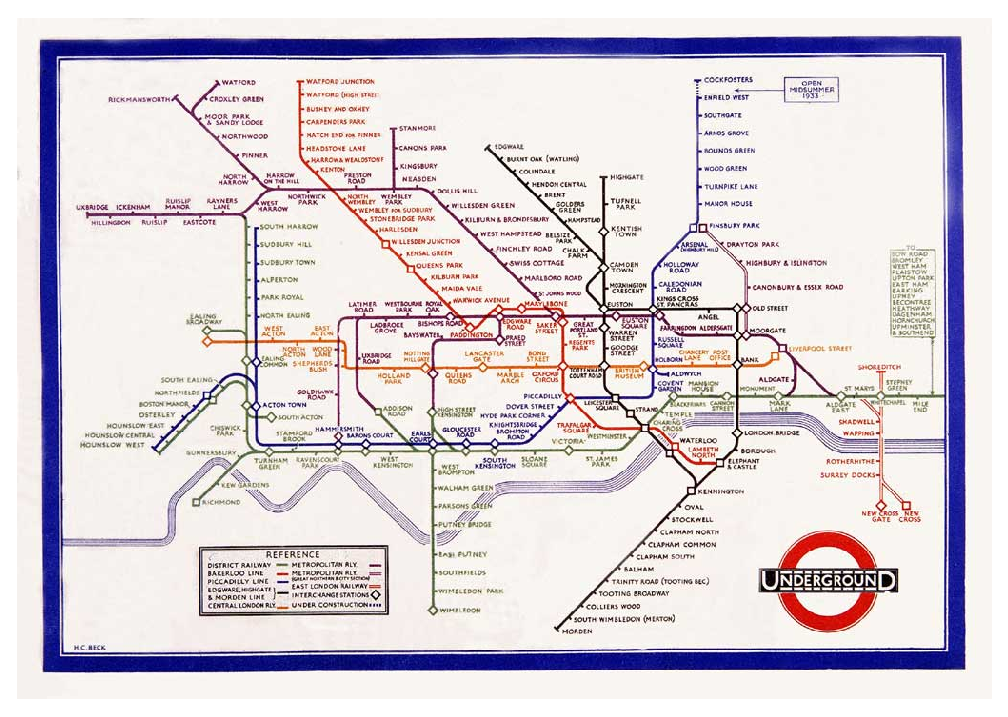
\includegraphics[width=0.9\textwidth]{beck_1933_map}
    \caption[1933 London Underground Tube map]{%
      The present Underground Tube map of London was introduced as early as
      1933 by graphic designer Harry Beck. It's merits are discussed
      in with regards to visual design by \citet{hadlaw03} and highlighted as
      a remarkable example of abstraction in relation to computing by
      \citet{kramer07}. Retrieved from the Transport for London web site:
      \url{http://www.tfl.gov.uk/beckmap1.jpg}}
  \end{center}
\end{figure}

No maps are available yet since the author don't have access to the required
\emph{Adobe Illustrator} software.

    \end{appendices}
  \backmatter
    \bibliographystyle{kluwer}
    \bibliography{bibliography}
\end{document}
